\documentclass{sigchi}

% Use this command to override the default ACM copyright statement (e.g. for preprints). 
% Consult the conference website for the camera-ready copyright statement.


%% EXAMPLE BEGIN -- HOW TO OVERRIDE THE DEFAULT COPYRIGHT STRIP -- (July 22, 2013 - Paul Baumann)
% \toappear{Permission to make digital or hard copies of all or part of this work for personal or classroom use is  granted without fee provided that copies are not made or distributed for profit or commercial advantage and that copies bear this notice and the full citation on the first page. Copyrights for components of this work owned by others than ACM must be honored. Abstracting with credit is permitted. To copy otherwise, or republish, to post on servers or to redistribute to lists, requires prior specific permission and/or a fee. Request permissions from permissions@acm.org. \\
% {\emph{CHI'14}}, April 26--May 1, 2014, Toronto, Canada. \\
% Copyright \copyright~2014 ACM ISBN/14/04...\$15.00. \\
% DOI string from ACM form confirmation}
%% EXAMPLE END -- HOW TO OVERRIDE THE DEFAULT COPYRIGHT STRIP -- (July 22, 2013 - Paul Baumann)


% Arabic page numbers for submission. 
% Remove this line to eliminate page numbers for the camera ready copy
% \pagenumbering{arabic}


% Load basic packages
\usepackage{balance}  % to better equalize the last page
\usepackage{graphics} % for EPS, load graphicx instead
\usepackage{times}    % comment if you want LaTeX's default font
\usepackage{url}      % llt: nicely formatted URLs
\usepackage{siunitx}
\usepackage{cite}
\usepackage{dblfloatfix}

% llt: Define a global style for URLs, rather that the default one
\makeatletter
\def\url@leostyle{%
  \@ifundefined{selectfont}{\def\UrlFont{\sf}}{\def\UrlFont{\small\bf\ttfamily}}}
\makeatother
\urlstyle{leo}


% To make various LaTeX processors do the right thing with page size.
\def\pprw{8.5in}
\def\pprh{11in}
\special{papersize=\pprw,\pprh}
\setlength{\paperwidth}{\pprw}
\setlength{\paperheight}{\pprh}
\setlength{\pdfpagewidth}{\pprw}
\setlength{\pdfpageheight}{\pprh}

% Make sure hyperref comes last of your loaded packages, 
% to give it a fighting chance of not being over-written, 
% since its job is to redefine many LaTeX commands.
\usepackage[pdftex]{hyperref}
\hypersetup{
pdftitle={Skintillates: Towards Epidermal Interactions},
pdfauthor={LaTeX},
pdfkeywords={SIGCHI, proceedings, archival format},
bookmarksnumbered,
pdfstartview={FitH},
colorlinks,
citecolor=black,
filecolor=black,
linkcolor=black,
urlcolor=black,
breaklinks=true,
}

% create a shortcut to typeset table headings
\newcommand\tabhead[1]{\small\textbf{#1}}
\newcommand{\ignore}[1]{}

%stop hyphenation
\tolerance = 1
\emergencystretch = \maxdimen

% End of preamble. Here it comes the document.
\begin{document}

\title{Skintillates: Towards Epidermal Interactions}

\numberofauthors{3}
\author{
  \alignauthor 1st Author Name\\
    \affaddr{Affiliation}\\
    \affaddr{Address}\\
    \email{e-mail address}\\
    \affaddr{Optional phone number}
  \alignauthor 2nd Author Name\\
    \affaddr{Affiliation}\\
    \affaddr{Address}\\
    \email{e-mail address}\\
    \affaddr{Optional phone number}    
  \alignauthor 3rd Author Name\\
    \affaddr{Affiliation}\\
    \affaddr{Address}\\
    \email{e-mail address}\\
    \affaddr{Optional phone number}
}

\maketitle

\begin{abstract}
Beyond phones, watches, and activity tracking devices, a new ecosystem of functional and fashionable wearable technologies can be easily, safely, and economically designed, prototyped, and integrated directly on the skin. Skintillates is a wearable technology that mimics tattoo - the oldest and most commonly used on-skin display in human culture. We demonstrate that by fabricating electrical traces and thin electronics on temporary tattoo paper, a wide array of displays and sensors can be created. Just like the non-functionalized temporary tattoo often worn by children to adults alike, the Skintillates devices flex naturally with the user's skin. Our simple fabrication technique also enables users to freely design and print with full range of colors to customize for their specific applications. In addition to demonstrating the technical capability of Skintillates in the application examples, we also briefly explore how they can serve as a platform for the combination of public and private body art and displayed data. (needs trim 6 words)
\end{abstract}

\keywords{
  Fabrications; wearable  \newline
}

\category{H.5.m.}{Information Interfaces and Presentation (e.g. HCI)}{Miscellaneous}

\section{Introduction}
\begin{figure}[!h]
\centering
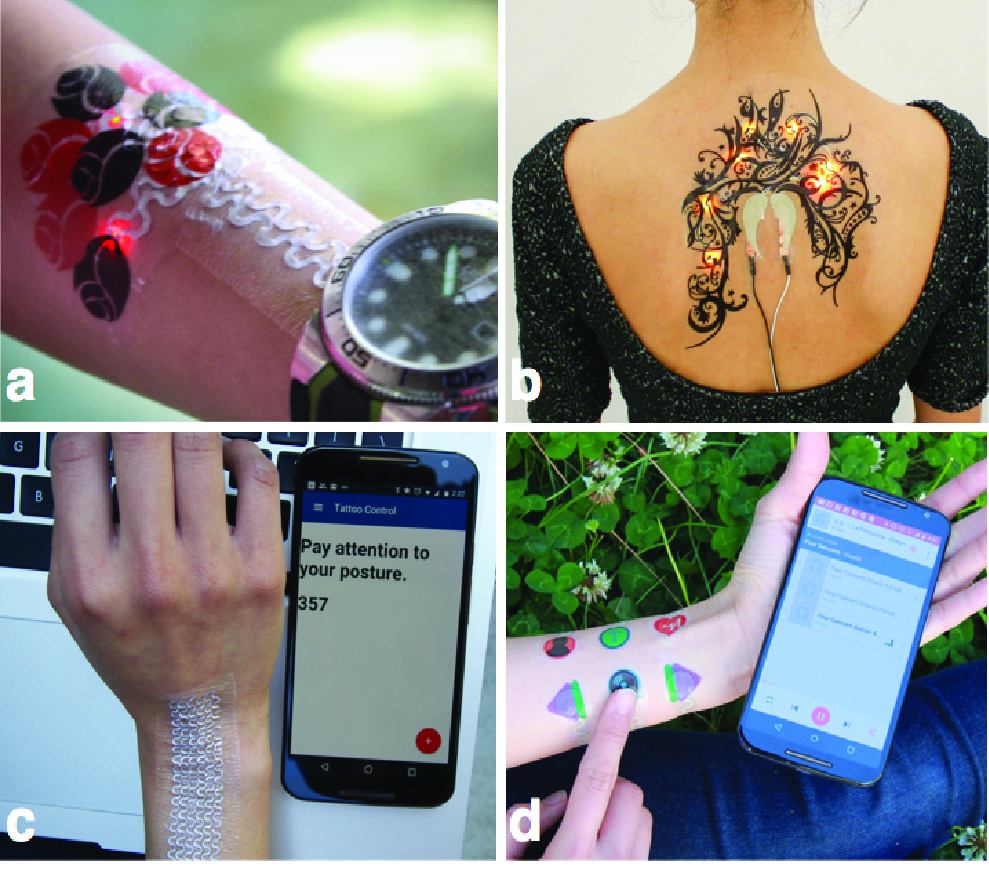
\includegraphics[width=1\columnwidth]{figures/Figure1}
\caption{Skintillates is a tattoo interactive platform that can be fabricated with an accessible process.}
\vspace{-8pt}
\label{fig:overall}
\end{figure}
Everyday, we interact with the world through our skin. The human skin senses important events that happen closest to us, and serves as an expressive medium when adorned with tattoo art. In this paper, we present Skintillates, a class of epidermal wearable interactive devices. Skintillate devices presented in this paper include electronic tattoos as passive and active on-skin displays, capacitive sensors for mobile device control and strain gauges for posture detection. Similar to traditional tattoos, Skintillates can be customized to be a variety of different shapes and colors to fit the user’s intended functions. Moreover, we demonstrate an accessible fabrication  method  for Skintillates that  uses  only  commercially-available materials and easy-to-obtain equipment. Skintillates is inspired by a line of research in micron-thin epidermal electronics pioneered by material scientists. Since these epidermal electronics directly contacts the skin, they can be made into extremely accurate, yet comfortable, sensors. However, due to existing devices intricate fabrication method, epidermal sensors remain to be a device mainly used in specialized medical and military applications. There is a clear need in the field of human-computer interactions for on-skin wearable electronics to enable natural and always-available interactions with the electronics and data around us\cite{MunehikoSato:2012we,chris:2011ve,ChrisHarrison:2010vi,DavidKim:2012uu,Harrison:2014ft,Laput:2014du}. In addition to giving commands using a wearable device, Skintillates can also serve as a programmable/addressable LED temporary tattoo display, on-skin sensor, or interactive control.(Fig.\ref{fig:overall}) 

\section{Motivation}
Our skin is a flexible, natural, and personal surface that affords a range of human interactions and expressiveness.  Our approach is to enable a new form of interaction and expression through temporary tattoos that can be easily designed, fabricated, attached, and comfortably worn.  In addition these devices should be durable, remaining functional for hours or even days. Beyond the technical design of our system, it is important to understand the historical, cultural, and deeply personal embedded meaning of tattoos and body art. 

\subsection{Towards Technological Tattoos: A Brief Cultural History}

Tattoos are known to have been part of human culture from as far back as the 4th millennium BC [cite] and used as forms of religious, tribal, and personal identification and adornment.  More recently, in the late 1950’s a “Tattoo Renaissance” emerged focused more on fashion and art. Today, with tattoos more common than ever, the desire for uniqueness and individuality in the designs has grown.  Similarly, the cultural milieu of technology has found itself more tightly integrated with tattoos. In just the past few years there have been QR code tattoos that provide interactivity through mobile phone apps and increasing adoption of temporary tattoos for changing fashion such as the Flash Tattoo [CITE]. 
Similarly, body modification by artists such as Stelarc reflect a movement toward the skin and body as expressive and interactive materials in relation to the cyborg and post human.  In a recent work Stelarc created a “functional” third ear on his arm using skin modification and wireless embedded electronics [cite].  Body Hacker Quinn Norton implanted a magnet under the tip of her finger enabling her to sense and interact with ferrous materials through her skin [cite].

The cultural role of the skin using permanent and temporary tattoos for personal expression aligns well with that of fashion and personal technology.  Mainly, how can such visual body elements become more interactive and expressive?


\subsection{Public and Private by Design:}
Tattoos serve a dual role as both a public messaging and more personal and often private embedding of meaning.  The user often controls the visibility of such designs directly through their choice and/or arrangement of clothing \cite{Doss:2009ee,McLeod:2014ua}. We view the flexibility and hybridity of these shifting public and private tensions as a desirable feature that we foreground in the design of Skintillates.   Like tattoos, Skintillates afford a wide range of personal designs varying in size, shape, color, body location, sensing, and electronic properties. We demonstrate and study examples of Skintillates as both public display and for private messaging in this paper. 

\subsection{Aesthetic and Personalization with Wearables}
Wearers of tattoos, both permanent and temporary ones, expect control of the aesthetic of the tattoos because body art sends a strong message about the wearer\cite{Doss:2009ee,McLeod:2014ua}. The message carried by a large vividly colored dragon tattoo versus a small white inside-arm tattoo is vastly different. However, most commercially available wearable systems offer color and few sizes as the only means to “personalize” their device. For example, buyers can choose the color of the most biomonitoring devices and smart watches, but for the most part the shape and functions of the device is predetermined. Counter to this limitation, Skintillates specifically decouple the visual aesthetic from the electronic functionally, enabling open, creative, and personal designs in an on-skin wearable device.

\subsection{Comfort, Safety, and Biocompatibility}
Any wearable, from clothing to electronics to tattoos must be safe and comfortable to wear for long periods.  Skintillates use materials that have been approved by U.S. Food and Drug Administration (FDA) for safe usage human skin. To minimize the possibility of negative skin-reaction to Skintillates, we used commercially available temporary tattoo paper as the substrate, and a medical electrode grade silver screen-printing ink as the conductive material for the circuitry\cite{Anonymous:6vWXbuD5}. 
%In one of the application examples, standard surface mount electronic parts are used. While most IC are made with inert materials that interact with skin, we hope to perform more studies or 

\section{Related Work}
Skintillates leverages a range of work across skin interaction research, flexible polymers, and epidermal electronics. (expand)
\subsection{Skin Interaction}
Expand - HCI related work - Chris Harrison's work (skin buttons, Skinput\cite{ChrisHarrison:2010vi,Laput:2014du}), implanted user interface \cite{Holz:2012ti}, Demonstrating the Feasibility of Using Forearm Electromyography for Muscle-Computer Interfaces [cite], skin drag display [cite]

\subsection{Polymeric On-skin Wearables}
The flexibility of polymer makes it a great substrate for wearable electronics. Great advances have been made in many applications, including robotic skin that can detect the touch of a fly via capacitive sensing\cite{Mannsfeld:2010is}, fully-functional on-skin keypads\cite{Anonymous:L82kTfjJ}, highly-stretchable strain gauge-based werable interface \cite{Boley:2014dr,Muth:2014bv}, ultra-flexible sensing circuits that include radio capability\cite{Jang:1gb,Anonymous:BBKIC9BZ}, and adaptive camouflage skin overlay\cite{Yu:2014ht}. The thickness and relatively high tensile modulus of polymeric wearable devices makes them durable and highly reusable, providing the ideal substrate for encapsulating complex electronics.

However, of the same properties that make polymeric wearables functional and reusable also often make them uncomfortable to wear for long periods since they are typically not very breathable on-skin without special device design \cite{Jang:1gb}. Moreover, to fabricate polymeric substrates that are uniformly thin for on-skin wearable applications, specialized, expensive equipment such as a spinner and vacuum chamber are often needed \cite{Son:2014iya,Yu:2014ht,Anonymous:BBKIC9BZ,Jang:1gb,Muth:2014bv,Anonymous:L82kTfjJ}. 

Additionally, incorporating conductive materials into polymeric wearables, mainly through mixing conductive materials with nonconductive polymer and injecting liquid metal into prefabricated channels, is non-trivial. Mixing a conductive material, such as graphite, into a nonconductive polymeric carrier is a simple process, but the resulting conductivity tends  to  be  extremely poor\cite{Weigel:2015fh}. Better electrically performing materials such as highly conductive liquid  metal  are unsuitable for on-skin applications such to their extreme toxicity \cite{Boley:2014dr}. These material limitations often make customizing the visual appearance of polymeric wearables difficult as well. One such example of a polymeric wearable device using this technique was iSkin, which addressed these problems by cutting the black graphite-functionalized conductive polymer into visually attractive patterns, thus cleverly turning the electrical layer into an aesthetically customizable layer \cite{Weigel:2015fh}. Skintillates seeks to expand on this work by broadening the visual design freedom by moving from purely monochromic art to a full range of inkjet printable colors. (this sentence needs work - stay nice!)

%The limitation of this technique lies in the lack of control over the color of the conductive polymer, thus reducing the visual design freedom of the wearable devices.

\begin{figure}[!h]
\centering
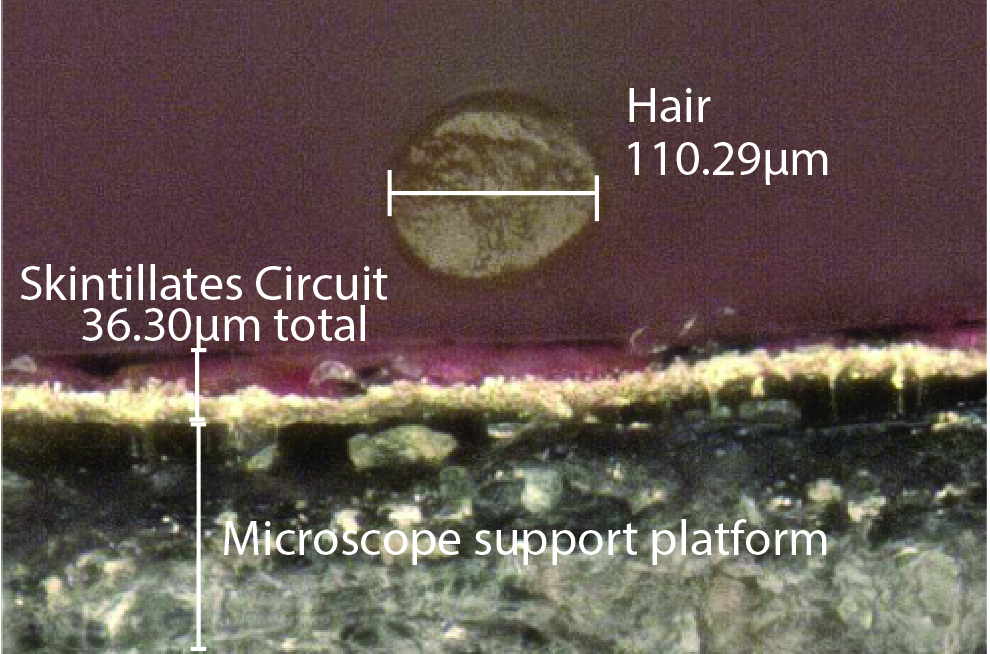
\includegraphics[width=1\columnwidth]{figures/Figure2}
\caption{A micrograph of the cross section of a \SI{36}{\micro\metre}-thick Skintillates device compared to a cross section of a piece of human
hair (\SI{110}{\micro\metre}).}
\vspace{-8pt}
\label{fig:micrograph}
\end{figure}
\begin{figure*} [!ht]
\centering
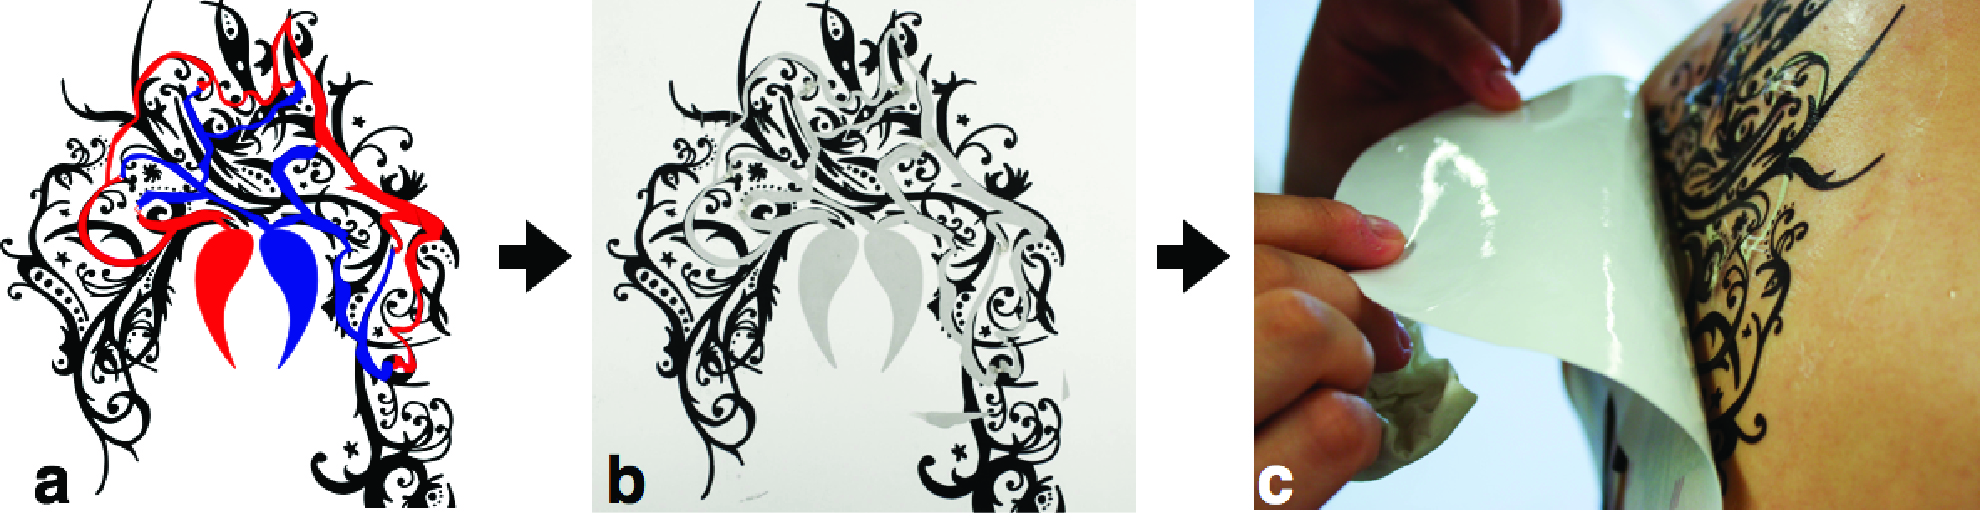
\includegraphics[width=1.0\textwidth]{figures/Figure3}
\caption{Application process.}
\vspace{-8pt}
\label{fig:applicationprocess}
\end{figure*}

\subsection{Epidermal Electronics}
Human skin has natural wrinkles, creases, and pits that are on the order of \SI{15}{\micro\metre} to \SI{100}{\micro\metre}\cite{Tchvialeva:2014wla}. If the wearable electronics have a thickness smaller or comparable to the natural skin features sizes, the wearer will not feel his/her skin unnaturally restrained\cite{Kim:2011bv}. The Epidermal Sensor, as defined by Professor John Rogers from University of Illinois at Urbana–Champaign, refers to the class of sensors with thickness on the order of natural skin wrinkles, conform to small skin movements such as wrinkling, and present minimal obstructions to users’ skin sensations\cite{Kim:2011bv}. Multifunction electronics, such as capacitive sensors that accurately detect physiological signals down to 0.5V, multilayer coils that enable on-skin RF communications, and strain and hydration sensors that aids in post-operation recovery\cite{Jeong:2013km,Kim:2014iq,Bandodkar:2014dl,Kim:2011bv}. %<-- Sentence Frag. This sentence is missing a verb or something?
Materials that are structurally stronger, such as polymeric stamp, water-soluble Poly(vinyl alcohol) (PVA), or skin-safe stickers are used as a structural backing to transfer the ultra-thin epidermal electronics devices onto the user's skin\cite{Son:2014iya}. Once transferred, the ultra-thin Epidermal electronics (most less than \SI{60}{\micro\metre}), with low Young's modulus that matches with human skin, can be attached to skin through van der Waals force alone\cite{Son:2014iya,Kim:2011bv}. 

Despite these the impressive scientific advances made by the development of epidermal electronics, the fabrication process makes them inaccessible to the general public. The flexibility of epidermal electronics enabled by the ultra-thin geometry that attaches to skin without substrate backing comes at the expense of complicated fabrication method and equipment, such as photoresist spinner, e-beam evaporator, mask aligner, chemical etch bay. The fine gold traces and electrodes (down to \SI{1}{\micro\metre} in width), and the ultra-thin conductive and insulation layers (ranges from 500nm to 5\SI{}{\micro\metre}), though extremely sensitive and conformal to the human skin, requires highly specialized lithographic equipment, high temperature metal deposition, and etching chemicals to fabricate\cite{Kim:2011bv,Kim:2014iq}. In one example application of Epidermal electronics, a small piece of temporary tattoo paper is used as a backing to transfer the epidermal device onto the user's skin\cite{Kim:2011bv}. Unfortunately, the etching process that fabricates the fine gold traces is incompatible with commercially available tattoo paper because the paper cannot withstand the chemical etchants, thus resulting an additional transfer step. Skintillates enables users to customize the device both electronically and aesthetically and be fabricated without cleanroom equipment or extreme temperatures. 


\begin{figure}
\centering
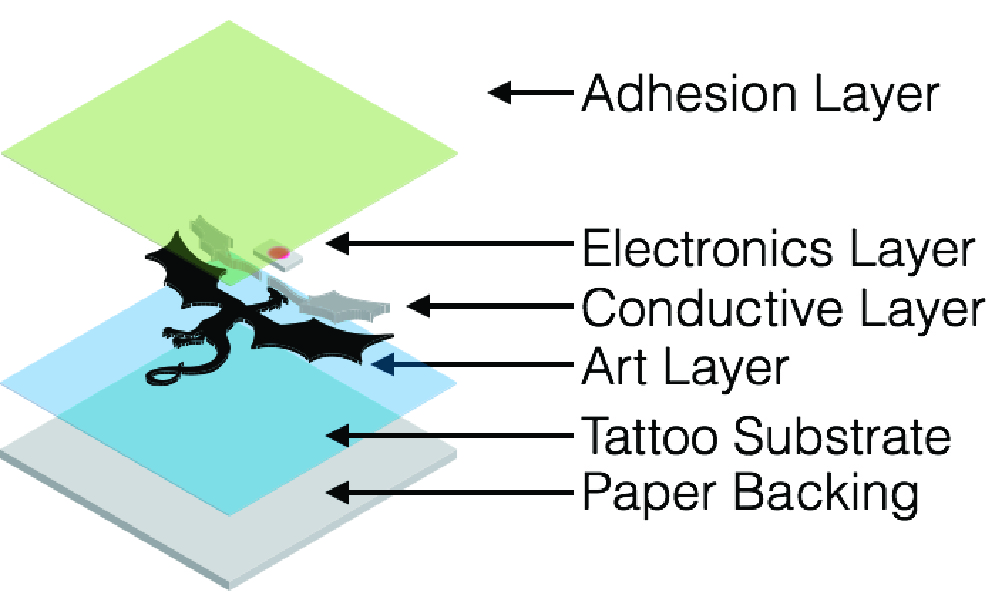
\includegraphics[width=0.9\columnwidth]{figures/Figure4}
\caption{An illustration of the different layers of a basic Skintillate device.}
\vspace{-8pt}
\label{fig:layers}
\end{figure}
 

\section{Fabrication}
(write intro to fabrication section)
\subsection{Material selection}
\begin{enumerate}
  \item The substrate has to be easily customizable to enable artistic expression with the temporary tattoo.
  \item The electronic has to be conductive enough to support basic functions for human computer interactions applications. 
  \item The tattoo must be easily applicable, stay on skin for a reasonable amount of time, and removable.
\end{enumerate}


Similar to epidermal electronics, we aimed for an integrated-with-skin tattoo aesthetic in Skintiallates. The amplitude of signals that we expect Skintillates to be used with for HCI applications are much larger than the signal strength of what epidermal electronics experiences (down to 500$\mu$V)\cite{Holleis:2008wn}. 
With these design considerations in mind, we chose to directly screenprint the circuits and electronics onto commercially available inkjet printable temporary tattoo papers. The silver ink used in this study was CreativeMaterials 118-38 Screen-printable ink, and the temporary tattoo substrates used is Silhouette Inkjet Printable tattoo paper. Although the  Skintillates devices, with conductive ink printed on top of temporary tattoo papers, are not as thin as epidermal electronics, it enables Makers to prototype on-skin interactive wearables with a much more accessible process. (Temporary tattoo papers are commonly used among crafters, it is therefore reasonable to assume that consumers find it acceptable to wear on skin although its not as conformable to skin as epidermal electronics.)(reword) Figure\ref{fig:micrograph} shows that a basic Skintillates device, which contains the tattoo substrate and a conductive layer, is approximately 36\SI{}{\micro\metre}, which is thinner than an average human hair. Users can inkjet print their own custom tattoo design, and screenprint the electronics with relatively inexpensive equipment. Screenprinting has also been shown to be able to create extremely fine and complicated electronic structures, and therefore this proposed fabrication method suitable for Makers of all skill levels and ages.

Due to the need to make a large number of Skintillates display and sensors in this project, we fabricated almost all of the Skintillates devices by screen-printing conductive ink. We have successfully created these devices with both conductive inkjet printing and conductive pens, but we will focus on the screen-print method in this paper. 

\subsection{Fabrication and Application Process}

\begin{enumerate}
  \item Design a nonconductive art layer with a graphic design tool of choice. Design the circuit and/or sensors to be screen-printed as the conductive layer. (Figure\ref{fig:applicationprocess}a)
  \item Use an inkjet printer to print the art layer design onto the tattoo substrate (still attached to the paper backing). 
  \item Cut a negative mask with vinyl cutter for screen-printing the conductive layer. 
  \item Apply vinyl mask onto the silkscreen. 
  \item Screen-print the circuit and/or sensors using the silver screen-printing ink.(Figure\ref{fig:applicationprocess}b)
  \item Let the ink dry in ambient temperature for 3-4 hours or 10 minutes in an oven at 100$^{\circ}$C. 
  \item Mount electronics onto the circuit using z-conductive tape at appropriate locations if needed.   
  \item Apply the adhesive layer that contains in the temporary tattoo paper package. 
  \item Put the Skintillate device on the desired body location. Wet and lift the paper backing (Figure\ref{fig:applicationprocess}c)
\end{enumerate}
An illustration of the Skintillates layers is shown Figure\ref{fig:layers}. LED's and resistors of the surface mount 0603 package, which has thickness of  \SI{500}{\micro\metre}, was used throughout this study to minimize increase in thickness in locations where electronics are mounted. Increased complexity in electrical functionality and aesthetic design could be achieved by using deviations of this basic fabrication method. The specific changes will be discussed in the application section. 

\subsection{Designing the Visual Appearance of Skintillates}
The visual appearance of Skintillates could be designed through the inkjet printable art layer and the conductive layer. Figure\ref{fig:design} shows a few examples of visual design possibilities. The color and shape of the art layer, which lies on top of the conductive layer when the tattoo is put on skin, can be used to hide or complement the conductive layer. A darker color printed on the art layer that completely overlaps the conductive layer can hide the conductive layer (fig\ref{fig:design}a). A lighter color printed on the art layer or a shape that does not completely overlap with the conductive layer allows the silver layer to peek through(fig\ref{fig:design}b). The shape of the functional silver conductive layer can also enhance the art layer by serving as a subtle decoration or a visual element in the design (fig\ref{fig:design}c-d). 

\section{Applications}
We envision a wide range of applications enabled by Skintillates and detail the technical designs and novel interactions across a set of examples in this section.

\subsection{On-skin Display}
\begin{figure}
\centering
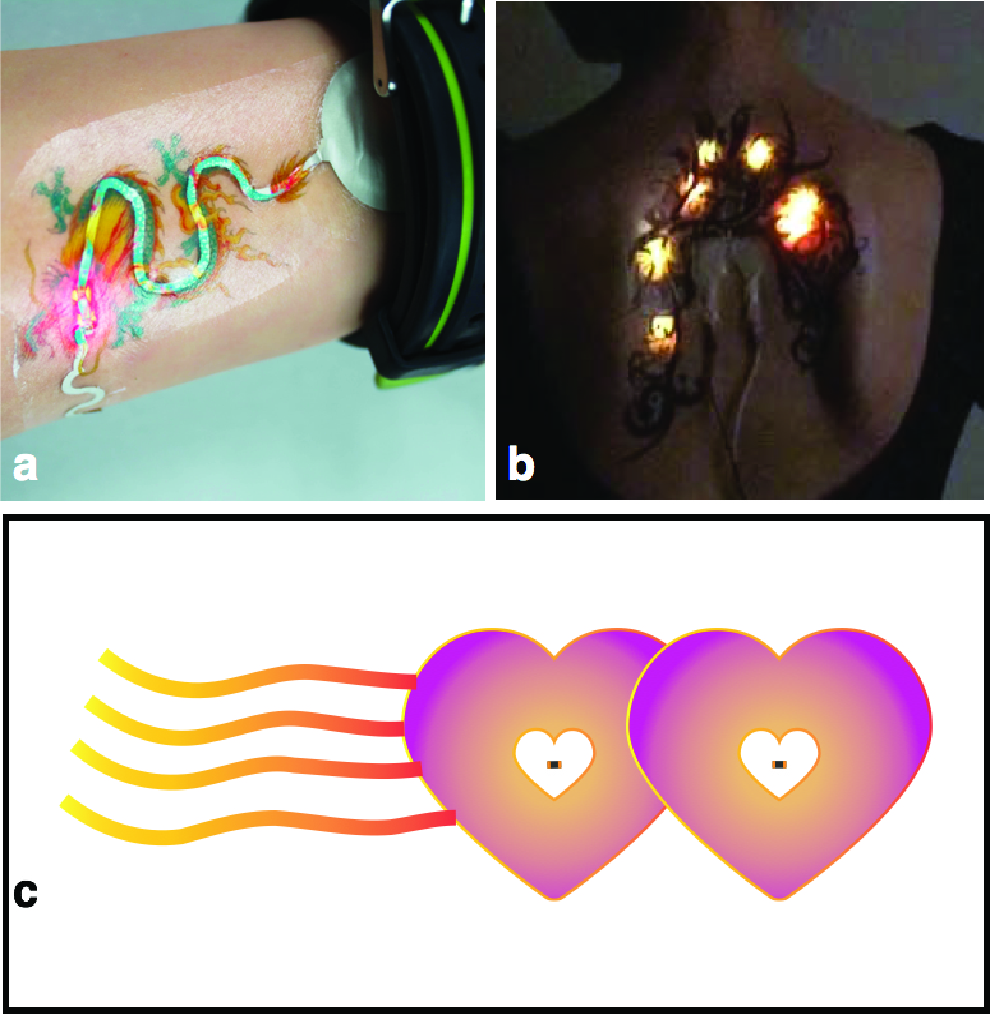
\includegraphics[width=0.8\columnwidth]{figures/Figure5}
\caption{Example of Skintillates tattoo displays}
\vspace{-8pt}
\label{fig:design}
\end{figure}

\begin{figure}
\centering
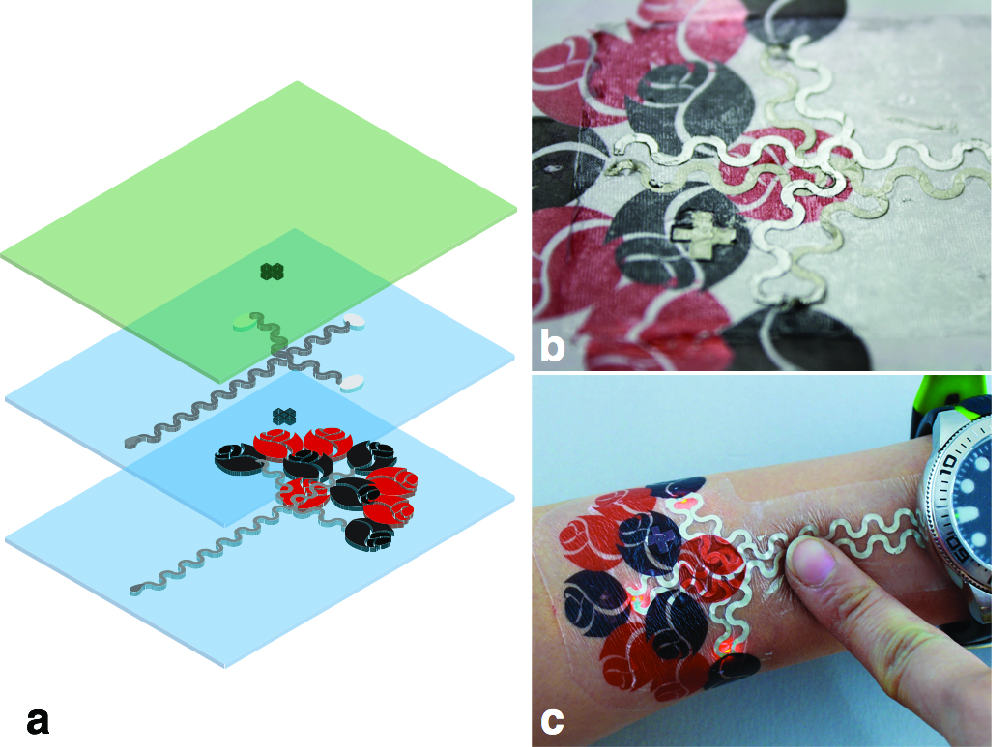
\includegraphics[width=1\columnwidth]{figures/Figure6}
\caption{Example of Skintillates tattoo displays}
\vspace{-8pt}
\label{fig:displays}
\end{figure}
One of the most important aspect of wearing tattoos, either temporary or permanent, is to express personal identity. 
Skintillates aims to augment the self-expression of tattoo artwork with electronics. In Figure \ref{fig:displays}, we show a few examples of decorative Skintillates public and private displays. Figure \ref{fig:displays}a shows a Skintillate dragon tattoo with red LED eyes that is electrically connected to the watch, and could potentially serve as a point-light display for a smart watch. Figure \ref{fig:displays}b demonstrates a back tattoo with LEDs that flash with music, which is controlled by an Arduino hidden under the wearers clothing. In this example, we also briefly explored the aesthetic of electronically functionally components on the tattoo. The power pads, which are traditionally circular or square in shape in printed circuit boards, are designed to look like wings to fit with the aesthetic of the art layer of the tattoo. In Figure \ref{fig:displays}c, we investigated the potential of using Skintillates as a private wearable display for intimate bio-data. We downloaded two sets of publically available test electrocardiogram (ECG) signals from PhysioNet to simulate the heartbeats from two people. In real-life applications, the Skintillates bio-data display can interface with biomonitoring data from commercially available wearable devices. The LEDs are programmed to blink as the signal strength reaches a certain amplitude, mimicking two heartbeats. The user wore the Skintillate ECG display under a shirt, which he/she can lift and glance at the private display when desired. In Figure \ref{fig:displays}d, we explore the possibility of incorporating Skintillate display with an existing tattoo. We omitted the art layer in this device and trace one of the tree branches with the silver ink to power three LED’s to light up the tattoo flowers.

\subsection{Multi-layer Display}
\begin{figure}
\centering
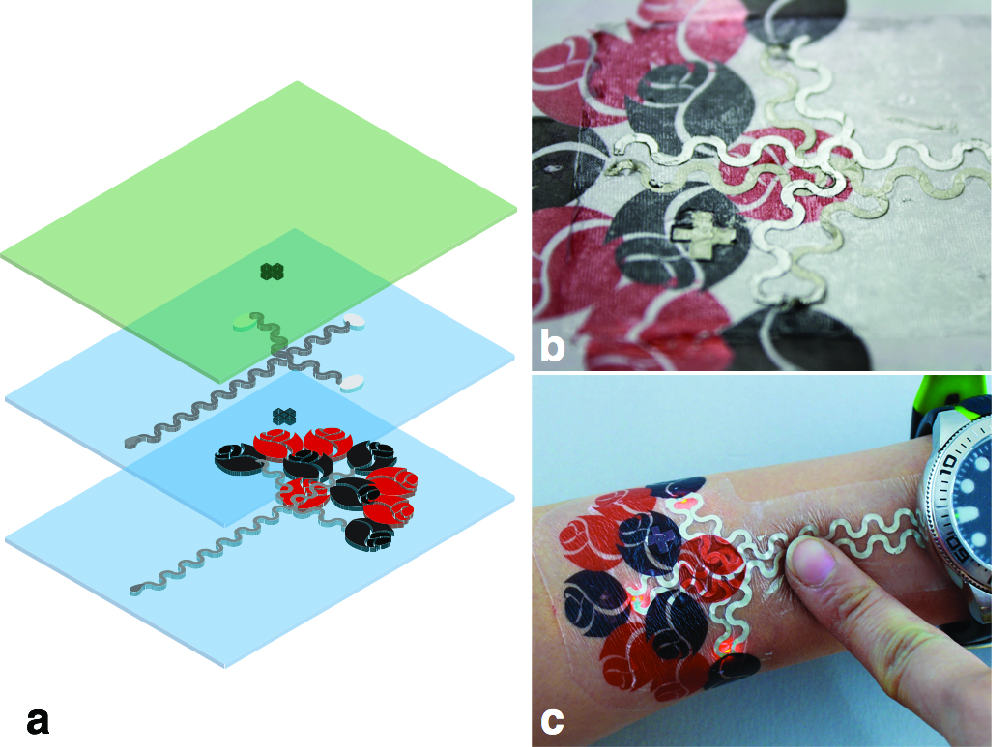
\includegraphics[width=1\columnwidth]{figures/Figure7}
\caption{Multilayer Display}
\vspace{-8pt}
\label{fig:multilayer}
\end{figure}

\begin{figure*}
\centering
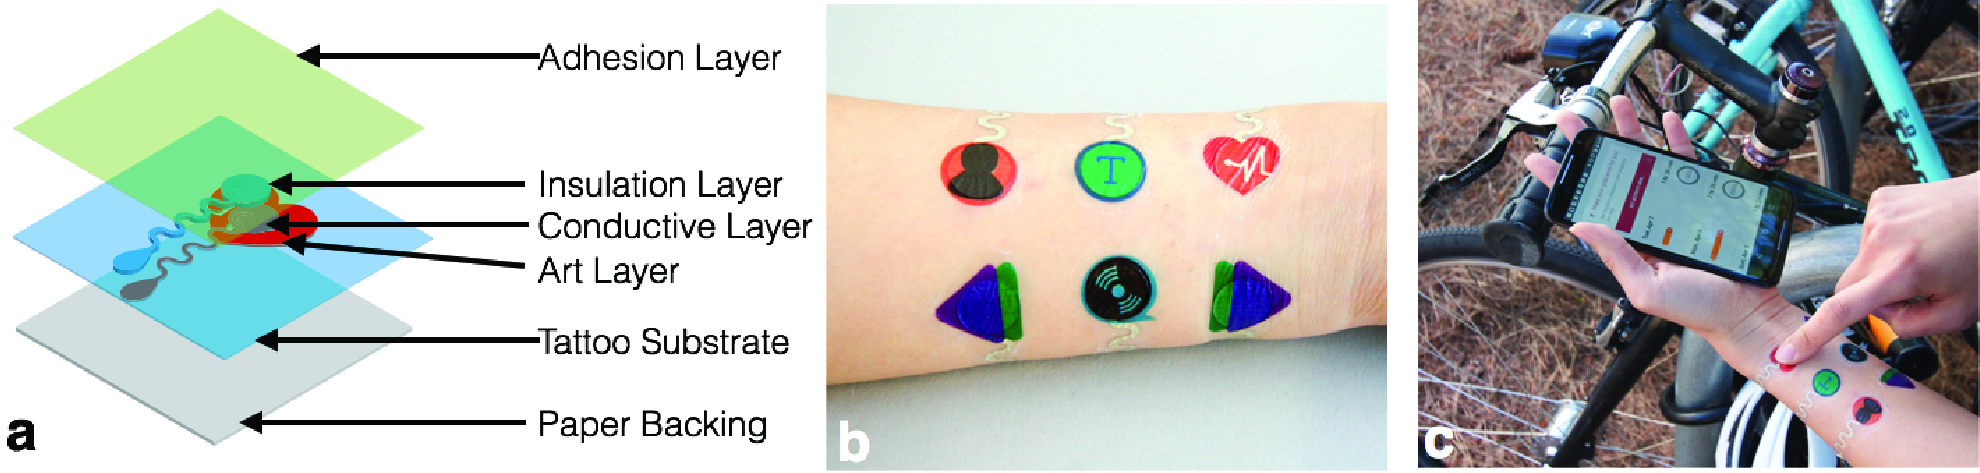
\includegraphics[width=1\textwidth]{figures/Figure8}
\caption{Capacitive touch sensing}
\vspace{-8pt}
\label{fig:capacitive}
\end{figure*}
Multilayer devices can be fabricated for aesthetic or electronic purposes. In printed circuit board design, multiple layers are often needed to achieve desired form and function. Epidermal electronics have also explored using multilayer device to support more complicated function. In arts practices, layers are often used as a mean to create dimensions. In order to fully explore combining arts and electronics on a wearable device, the Skintillates fabrication process should be able to support electronic function and aesthetically attractive multi-layer devices. Figure \ref{fig:multilayer}a shows an exploded view of a multilayer Skintillates device. In this study, we created a second conductive layer, but the same procedure could be used for creating a second art layer. A second layer was screen printed on a separate temporary tattoo substrate, and was released from the paper backing onto the first conductive layer. In order to electrically connect the first and second conductive layers, we created vias by cutting holes in the substrate at appropriate locations. Figure \ref{fig:displays}b shows a closed-up image of the dual-layer Skintillate device. The top layer traces are insulated from the bottom layer traces with a tattoo layer substrate, and vias are opened at the end of the traces to allow the LED's to make contact with both sets of the traces. Although the multilayer Skintillates devices are thicker than the single layer devices, they remain reasonably flexible on skin. In figure\ref{fig:displays}c, we show that the dual-layer Skintillates device remain operational even when the traces are being compressed with the skin. 


\subsection{Capacitive Touch Sensing}

Advanced sensing, including capacitive sensing, using epidermal devices is well-established. In many research studies, various algorithms, data processing methods, and grounding schemes are utilized to overcome any technical difficulties usually associated with wearable sensing.  Through careful material selections, we can achieve sensitivity suitable for common interactive applications. As mentioned in the Fabrication section, the silver screen printing ink (or most of the silver ink on the market) is very conductive (0.5$\Omega/\square$). 
 The high conductivity is important in resistive switch design, where the touched surface needs to be conductive enough to close the switch; it is also pertinent in capacitor design, where the availability of charge directly affects the sensitivity of the capacitive button (Gauss’s law=$\frac{\sigma}{\epsilon}$). In the following sections, we will go through a few sensing examples using the Skintillates devices. 


Capacitive sensing is ubiquitous in interaction design - from sensing gestures to sensing direct touch, the change in electric field carries rich information about the space around us. Such sensing allows Skintillates to easily incorporate capacitive buttons that can be used as local input or as remote signals to control a mobile smartphone. To ensure reliable performance of the capacitive sensor, both the electronic filtering and the physical device insulation have be carefully designed. To reduce cost and simplify the design the raw data of the capacitive sensor is processed and filtered by a commercially available breakout board\footnotemark. To insulate the capacitive sensor against the skin where it is attached, we modify the fabrication steps slightly by adding insulative temporary tattoo substrates without any silver conductive ink on top of the conductive electrodes. This insulative layer prevents electric charges from the surface of the skin to interfere with the desired capacitive touch signal (Fig.\ref{fig:capacitive}a). The capacitive buttons control various mobile smartphone applications (i.e. music, social media, etc) through a low power wireless bluetooh module\footnotemark. By placing the Skintillates in the inside of the user’s arm (Fig\ref{fig:capacitive}b), he/she can control the mobile applications on an easily accessible body location (Fig\ref{fig:capacitive}c). The size and shape of the Skintillates buttons are highly customizable, enabling visual design freedom - such as creating buttons with shapes that represent the application being controlled, and electronic design freedom - such as capacitive sliders and wheels.

\footnotetext{Adafruit Capacitive Touch Sensor Breakout MPR121 connected to an Arduino Uno}
\footnotetext{A low-power BLE module provided connectivity to the phone.}

\subsection {On-skin Resistive Sensor}
\begin{figure}
\centering
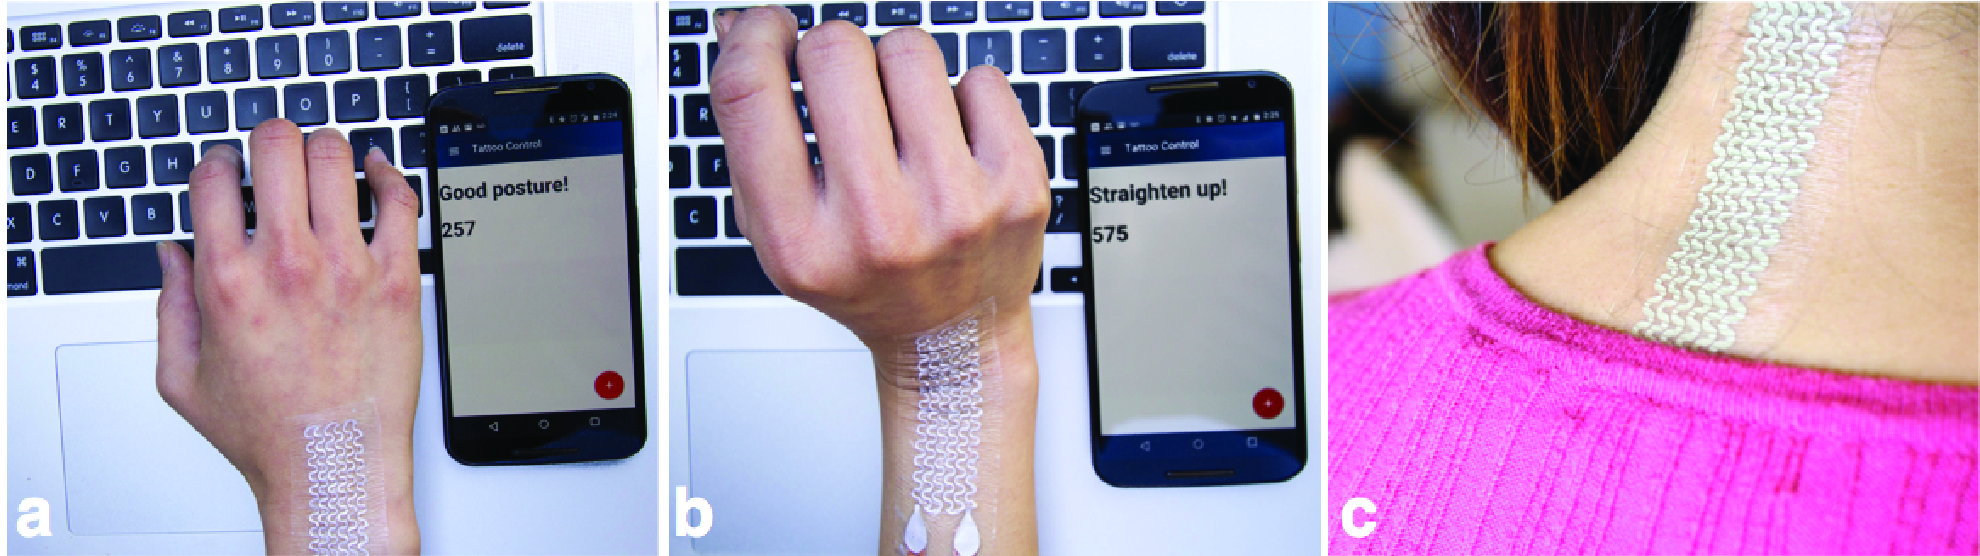
\includegraphics[width=1\columnwidth]{figures/Figure9}
\caption{Example of Skintillates tattoo displays}
\vspace{-8pt}
\label{fig:figure8}
\end{figure}
Using the human body as a conductor to form a closed circuit to turn on a light is common science experiment, and this sensing method can also enable interesting interactions - such as turning bananas into switches - made popular by MakeyMakey. We demonstrated that Skintillates can be used as a resistor sensor that is compatible with MakeyMakey. The construction of the Skintillates resistor sensor is very similar to that of the capacitive sensor, with an insulative layer beneath the electrode to prevent electrically connection between the sensor and the skin that it is attached to. Figure 8a shows two Skintillates sensors shaped as kites, which are connected to the MakeyMakey to act as the left and right arrow of a computer keyboard. The custom buttons are then used as a controller to play a computer game of moving the kite up and down to avoid hitting objects in the sky. A huge library and community support are available for prototyping with MakeyMakey, and the Skintillates resistive sensor can be used to enable a wide range of wearable interactions. 
\subsection {Strain Gauge}
\begin{figure*}
\centering
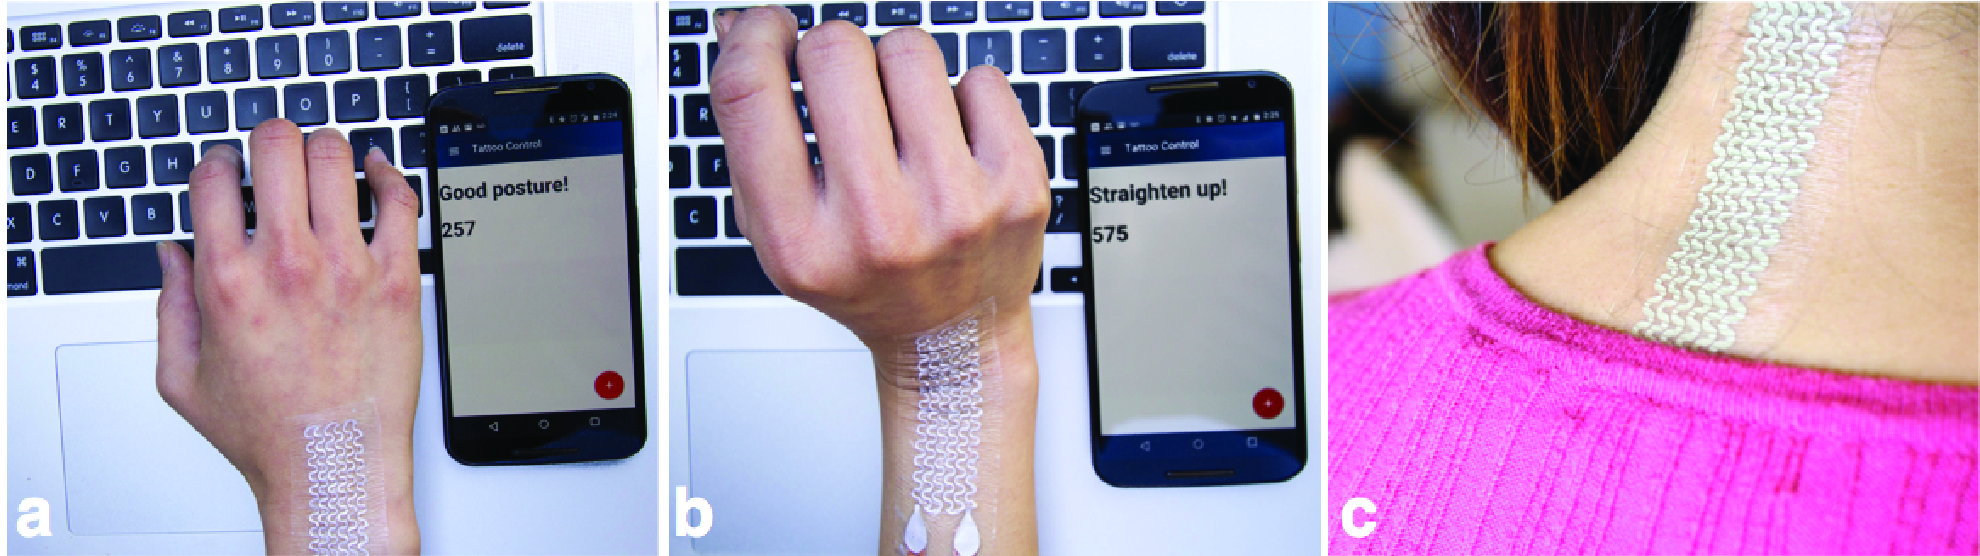
\includegraphics[width=1.0\textwidth]{figures/Figure10}
\caption{Strain gauge for posture sensing}
\vspace{-8pt}
\label{fig:figure9}
\end{figure*}
The subtle analog motions of the human body carries information that goes beyond the digital on/off button. The Skintillates strain gauge captures the fluid motion of the human body by translating the movement into a variable resistance. %[I think "fluid motion" gives the wrong connotation, when one first reads this, like its tracking bodily fluids or something.]Skintillates strain gauge captures the full range of human motion by translating muscle movements into a variable resistance. Valid, but I like the image of "fluid motion". Let me think about this more.
 The strain gauge has a longer length in the direction of the wrist bending during typing. As the sensor stretches with the wrist, the resistance becomes higher proportionally. The change in resistance is detected through a wheat stone bridge and amplified using the INA125P operational amplifier. Before amplification, the variation in the resistance ranges from 37$\Omega$(when wrist is flat) to 54$\Omega$ The amplified analog value is read using an Arduino Uno and transmitted to a mobile phone via bluetooth. 
 The value is then displayed on the screen of the mobile phone, and the appropriate warning messages are displayed as the user’s wrist posture change. Although the strain gauge is applied on the wrist in this example, similar application can also be used for back posture by placing the sensor on the neck (Figure 7c). In addition to posture detection, Skintillates strain gauge can serve as an always-available sensor to detect different gestures for electronic interactions or be incorporated into performance art. 

\section {User Study}
\begin{figure}
\centering
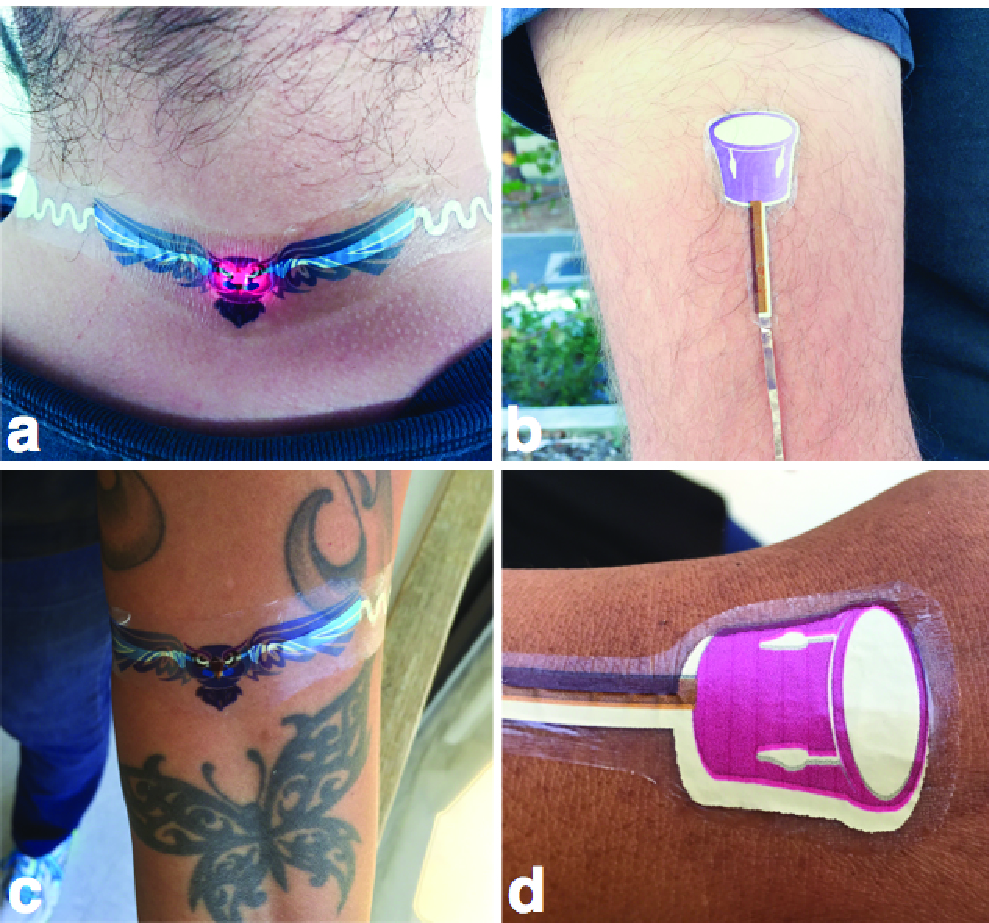
\includegraphics[width=1\columnwidth]{figures/Figure11}
\caption{Example of Skintillates tattoo displays}
\vspace{-8pt}
\label{fig:userstudy}
\end{figure}
In order to study the user experience of the Skintillates devices, we recruited 10 participants (mean age 29.7) to each wear 1) a Skintillate display measures 6.5 in x 1.0 in and connected to a 3.3V coin cell battery, 2) a Skintillate resistive sensor measures 1.3 in x 0.8 in, and 3) two temporary tattoo without any conductive layer as controls. Participants were free to apply the Skintillates devices on a body location of their choice with the restriction of placing the control tattoos close to the display and the sensor,  and they were asked to wear the devices for the duration of a work day (ranges from 8-10 hours). During which they performed their normal work functions, which mostly includes office activities such as typing, writing, and manipulating light machinery. At the end of the work day, participants were surveyed about their qualitative and quantitative opinions about the Skintillates devices. The functionality of Skintillates devices were tested to assess durability and participants were free to choose whether they want to keep wearing the devices. On the next day, participants were given another survey about the social aspect of Skintillates.


The majority of the users chose to put the Skintillates devices on their arms, while one user placed the Skintillates display on the back of the neck. When asked about their decision of the placement of the Skintillates devices, users cited the shape of the Skintillates devices and their outfit of the day to be the main drivers. In the follow up survey, user were asked about how long they kept wearing the Skintillates devices after they were given the choice to take them off. All of the participants (8 out of 10) who have plans to interact with friends and family after the work day kept wearing the tattoo after the study so that they can show the Skintillates devices to their loved ones - ``I wanted to keep it because I thought my kids would think that this is the coolest thing ever''. Two of the participates mentioned that although he/she did not have prior plans to go out after work that night, they decided to go to a public place (one to a restaurant for take-out, and one to a sports bar) to show off the Skintillates display. R7, who went to a sports bar to show off the tattoo, reported ``it seems to be a waste not to show this to someone''. When asked to imagine potential applications that they would like to use the Skintillates devices for, many applications were around instant and unexpected interactions with their surrounding electronics (``a henna tattoo that can control everything in my house'', ``tattoo buttons that make people massage my back when they need to turn on the light'', ``control things with Spiderman gesture''), decorative body display (``put some evil red eyes on my skull (permanent) tattoo'', ``burning man costume''), and functional body display (``turning signal for motorcyclists'', ``a red/green light for when I want to be bothered by people''). 

Participants were asked to rate the wearing comfort of the Skintillate display with and without consideration of the battery connection (i.e. copper tape connected to the battery). The authors recognize the limitation of this study was that different locations of the skin have different nerve endings and can affect the comfort level - however, we were more interested in learning how users would use the Skintillates devices on a body location of their choice in this study. The wearing comfort of the control temporary tattoo 9.1/10. Without considering the battery connection, the wearing comfort of the Skintillates display and resistive sensor have an average rating of 8.2 and 8.8 out of 10 respectively. Most participants describes Skintillates devices as something that they ``don't even feel after a while'' and ``feels very similar to a normal temporary tattoo'', and the small 0.5mm-thick 0603 electronic parts as ``little bumps'' and do not significantly affect wearing comfort. When considering the battery connection, the wearing comfort of the display decreased to an average rating of 7.1/10. Participants were most bothered by the battery connections and the hard coin cell battery. One out of ten Skintillate displays was damaged due to a strong tear and separation between the connection wires and the Skintillates device, and all the rest of the nine displays remained perfectly functional at the end of the study.

All participants reported that they would like to wear the Skintillates device again, as well as express desires to design their own Skintillates displays and sensors. Although all of the participants took off the Skintillates devices before showering or going to bed, all of them said that they took the devices off very carefully as to not damage them. In particular, all of the participants kept the display devices for reuse. 

\ignore{potentially interesting descriptions of the resistive sensor: 
it's like your skin can control things in the house 
can you make a air guitar with sensors on your finger

potentially interesting application of the resistive sensor: 
make a spider man thing
let's put the sensor on your neck - let's put a bone conduction microphone on the back of your neck (omg how engineer is this)

potentially interesting descriptions of the display: 

potentially interesting application of the display: 
make the display a turn signal for motorcyclists
Burning man! (i'm going to die if i get one more burning man comment)
a pretty baby monitor(from the new dad)
a red/green led to show people whether you want to be bothered at the moment
hook up to sensors to show hydration level (why is everyone freaking out about not drinking enough water??)


(This didn't happen to much because most people went straight home. There were only 4 uninitiated conversation)
In a few of the conversations about the Skintillate devices in which the participants did not initiate, the dangling battery wires were the starting point of conversations. (The other half of initiated by the ``lit-up tattoo'', unsurprisingly.) One participant recounted a conversation happened with a stranger in an elevator, where the stranger initiated the interaction by saying ``are you hooked up to something on your arm''. The dangling wires serves as something that people are somewhat familiar with to strike up a conversation about the novel Skintillates displays.

}

\ignore{Why did you take it home? How long did you keep it on. Who did you show it to. Did you have any public experience. How did you fit this into your daily life? 
Every place: 
Upper arm 
During the course of wearing this, what else would you use it for. Sensing? 
Would you wear this again. Would you wear this on a different location?  

Skintillates was also invited to participate in the two-day exhibition of the National Maker Faire 2015. During which Skintillates LED displays powered by coin cell batteries were given out as part of the exhibit. The LED displays were customized to be a LED lit-up Maker Faire logo, as requested by the event organizer. Users mostly chose to wear the devices on the top of their arms and the outside of their lower legs. The devices were met with great enthusiasm and generated many inspiring conversations. In particular, the displays worn by the event organizer led many Maker Faire participants and potential academic collaborators to visit our booth and offer application suggestions such as displays for events like Burning Man, medical electrodes for children, or custom motion controller for robots.} 


\section {Limitations}
Although Skintillates provides tremendous new features and benefits to creating novel wearable electronics, there are several limitations. First, although the Skintillates device is highly flexible, the electrical connection, currently made with copper tape, is not. In additional to creating discomfort, the difference in material  properties causes the electrical connection to be the mechanically weakest point of the device. This problem can be overcome by stabilizing the connection using a small piece of medical-grade tape - the tape relieve most of the stress exert on the connection and prevent tearing of the connection. In future work, we would like to develop a flexible electrical connector that can move with the skin and provide an electrical interface with the Skintillate device. 

Another limitation lies in the reusability of the Skintillates devices. In the research team's experience, the Skintilltaes devices can be reused at least four to five times if the devices contains finely traced (\textless 2mm) circuits and many more times if the for sensors with large conductive patches. The reusability of the devices could potentially be improved with a thin (<10um) spray-on encapsulating layer. Further studies can also be performed to optimize the electronic design for durability. 

\section {Discussion and future applications}
The development of Skintillates has significant impact in customizable flexible and wearable electronics and their applications. The simple fabrication process of Skintillates provide an alternative to prototyping with 3D printing or polymer casting and curing.  The design freedom, in terms of electronic, functionality, and visual aesthetic, of Skintillates can support a diverse ecosystem of users from diverse backgrounds, including engineers, designers, and artists. We plan to continue investigating creating more complex interactive electronics on Skintillate devices and studying how these devices can blend artfully and seamlessly into people's daily lives. Moreover, we would like to explore the possibility of incorporating Skintillates displays and sensors into performance arts. 

\section {conclusion}
In this paper, we have presented our Skintillates, a family of novel wearable devices that can be fabricated with easily accessible materials and equipment. 
 \cite{Kim:2015ii}.



%\section{Acknowledgments}

%We thank CHI, PDC and CSCW volunteers, and all publications support
%and staff, who wrote and provided helpful comments on previous
%versions of this document.  Some of the references cited in this paper
%are included for illustrative purposes only.  \textbf{Don't forget
%to acknowledge funding sources as well}, so you don't wind up
%having to correct it later.

% Balancing columns in a ref list is a bit of a pain because you
% either use a hack like flushend or balance, or manually insert
% a column break.  http://www.tex.ac.uk/cgi-bin/texfaq2html?label=balance
% multicols doesn't work because we're already in two-column mode,
% and flushend isn't awesome, so I choose balance.  See this
% for more info: http://cs.brown.edu/system/software/latex/doc/balance.pdf
%
% Note that in a perfect world balance wants to be in the first
% column of the last page.
%
% If balance doesn't work for you, you can remove that and
% hard-code a column break into the bbl file right before you
% submit:
%
% http://stackoverflow.com/questions/2149854/how-to-manually-equalize-columns-
% in-an-ieee-paper-if-using-bibtex
%
% Or, just remove \balance and give up on balancing the last page.
%
\balance

\bibliographystyle{acm-sigchi}
\bibliography{skintillates}
\end{document}
